%\def\year{2017}\relax
%%File: formatting-instruction.tex
\documentclass{article}
%\usepackage{aaai17}
\usepackage{ijcai17}
\usepackage{times}
%\usepackage{helvet}
%\usepackage{courier}


%\usepackage{url}
%\usepackage{color}
%\usepackage{latexsym}
\usepackage{epsfig}
\usepackage{graphicx}
%\usepackage{booktabs}
%\usepackage{diagbox}
%\usepackage{array}
%\usepackage{multirow}
%\usepackage{multicol}
%\usepackage{hhline}
%\usepackage{pbox}
%\usepackage{threeparttable}
%\usepackage{epstopdf}
\usepackage{amsmath}
\usepackage{amssymb}
\usepackage{amsthm}
\usepackage{algorithm}
\usepackage[noend]{algpseudocode}
\usepackage[small]{caption}

%\providecommand{\e}[1]{\ensuremath{\times 10^{#1}}}

\newtheorem{definition}{Definition}

\newcommand{\figref}[1]{Figure \ref{#1}}
\newcommand{\tabref}[1]{Table \ref{#1}}
\newcommand{\secref}[1]{Section \ref{#1}}
\newcommand{\eqnref}[1]{Eq. (\ref{#1})}
\newcommand{\defref}[1]{Def. \ref{#1}}
\newcommand{\algoref}[1]{Algorithm \ref{#1}}

\newcommand{\KZ}[1]{\textcolor{blue}{Kenny: #1}}
\newcommand{\KQ}[1]{\textcolor{red}{Kangqi: #1}}
\newcommand{\XS}[1]{\textcolor{blue}{Xusheng: #1}}


%\newcolumntype{I}{!{\vrule width 1pt}}
%\newlength\savedwidth
%\newcommand\whline{\noalign{\global\savedwidth\arrayrulewidth
%                            \global\arrayrulewidth 1pt}%
%                   \hline
%                   \noalign{\global\arrayrulewidth\savedwidth}}
%\newcommand\BibTeX{B{\sc ib}\TeX}
%
%\frenchspacing
%\setlength{\pdfpagewidth}{8.5in}
%\setlength{\pdfpageheight}{11in}
\pdfinfo{
/Title (A Data-Driven Approach to Infer Knowledge Base Representation
        for Natural Language Relations)
/Author (Kangqi Luo, Xusheng Luo, Xianyang Chen, Kenny Q. Zhu)}
\setcounter{secnumdepth}{2}

\begin{document}
% The file aaai.sty is the style file for AAAI Press
% proceedings, working notes, and technical reports.
%

%\title{Paraphrasing Natural Language Relations to Knowledge Base Schemas}
%\title{A Data-Driven Approach for Representing Natural Language Relations by Knowledge Base Schemas}
\title{A Data-Driven Approach to Infer Knowledge Base Representation \\
	for Natural Language Relations}

\author{
Kangqi Luo,\hspace*{3mm} Xusheng Luo,\hspace*{3mm} Xianyang Chen,\hspace*{3mm} Kenny Q. Zhu$^*$\\
Shanghai Jiao Tong University, Shanghai, China\\
\{luokangqi,freefish\_6174,st\_tommy,kenzhu\}@sjtu.edu.cn
%AAAI Press\\
%Association for the Advancement of Artificial Intelligence\\
%2275 East Bayshore Road, Suite 160\\
%Palo Alto, California 94303\\
}

\maketitle
\begin{abstract}
This paper studies the problem of discovering the structured knowledge representation of binary natural language relations.
The representation, known as the schema, generalizes the traditional path of predicates to support more complex semantics.
We present a search algorithm to generate schemas over a knowledge base, and propose a data-driven learning approach to discover the most suitable representations to one relation.
Evaluation results show that inferred schemas are able to represent precise semantics, and can be used to enrich manually crafted knowledge bases.~\footnote{Kenny Q. Zhu is the contact author and is partially
supported by NSFC grants 91646205 and 61373031.}


%as well as support natural language question answering.
\end{abstract}

%relation instance | relation triples | entity pairs

%learned | paraphrased

\section{Introduction}

Protein$-$protein interactions (PPIs) are of central importance for the majority of biological functions, such as signal transduction, metabolic pathways, molecular dynamics, and protein networks\cite{Hoffmann.Krallinger.ea:2005}, for they serve as the most fundamental building blocks of the entire interacademic systems of any organisms. Collecting data on pairwise interaction relationships is essential for multiple purpose, including identification of modules with certain functionality\cite{Spirin.Mirny.03}, mapping diseases to dominated genes\cite{Ideker.Sharan.08}, and after all, understanding wholistic metabolic/genetic networks from a system biology perspective.

A lot of databases have been built to store protein and genetic interactions from major model organism species and are available in various standardized formats, such as MINT\cite{Zanzoni.Montecchi-Palazzi.ea:2002}, BIND\cite{Bader.ea:2003}, BIOGRID\cite{DBLP:journals/nar/StarkBRBBT06}, etc. Among those mainstream databases, the data largely rely on voluntary reports by scientists or researchers, besides, comprehensive curation efforts become indispensable for the sake of accuracy. However, the amount of biology-related literatures with respect to protein interactions grows explosively and thus make it either impossible or impractical to manually detect PPI information anymore.

Considering huge amount of PPI information with great wealth hidden in published papers, in recent years, numerous mining techniques have been proposed that aim to extract PPI information automatically from free text, especially machine learning, information retrieval, and natural language processing\cite{DBLP:journals/bib/WinnenburgWPDS08}.These approaches can be roughly categorized into three classes: co$-$occurrence, rule$-$based, and machine learning. 

Co$-$occurrence is the approach with most simplicity and naivete. Just as its name implies, this method intends to find out pairs of proteins that co-occur in the same context. The scope of "same context" ranges from phrase, sentence, paragraph to whole abstract, even document. The underlying assumption is that whenever two proteins are mentioned together by authors, chances are high that there is some kind of relationship between them. However, however, in-context closeness even semantic relation does not necessarily represent actual biological interaction. As a consequence, a large fraction of candidate pairs are mismatched inevitably, causing a high recall but low precision.

The second approach is rule-based extraction, in other words, pattern matching. There are many types of rules, most of them concern natural language processing (NLP). One way is to specify hand-crafted regular expressions before hand, which mostly lean on language usage preference. Besides, by using full or partial (shallow) parsing strategies, more information would be acquired, such as part-of-speech taggers, local dependencies between syntactic components, context-free grammar\cite{DBLP:journals/bioinformatics/TemkinG03}, and full sentence structure. Compared to co$-$occurrence, rule-based approach enjoy better precision but much lower recall. In addition, since the rules are usually derived from training data, that is to say, the improper choice of training data would be significantly lethal, therefore quality of extraction is invariably instable and may not applicable to other data.

The third and most commonly used approach use machine learning techniques, in this case, the task to extract protein$-$protein interactions turns out to be a binary classification problem. Each protein pairs are represented along with a set of features, which is associated with their context, then a well$-$defined classifier gives the answer whether the candidate protein pairs is classified to be qualified PPI. (TO BE FURTHER FILLED!!!)

In this paper, we introduce a general bootstrapping framework for Protein$-$protein interaction extraction from natural text.Our method differs from most of the previous works in three aspects:

(1)The extraction process is driven by only tiny fraction of training data, which are regarded as seed data. In each round, it would derive reliable patterns automatically from seed data, then extract more positive PPI pairs consequently, what's more, the seed data would be augmented by the newly extracted results with high confidence.

(2)multiple graph kernel. 

(3)various evaluation.





\section{Problem Definition}
\label{sec:problem}

In this section we formally define the problem of short title extraction.
A char is a single Chinese or English character.
A segmented word (or term) $x$ is a sequence of several chars such as 
``Nike'' or ``牛仔裤''(jean).
A product title, denoted as $X$, is a sequence of words $\{x_1, x_2, ..., x_n\}$.
Let $Y$ be a sequence of labels $\{y_1, y_2, ..., y_n\}$ over $X$, where $y_i \in \{0, 1\}$.
The corresponding short title is a subsequence of $X$, denoted as $S = \{x_i\}$, 
where $y_i = 1$ and $|S| \le n$.

%we are interesting in obtaining a short title which can represent the most important information about the product.

We regard short title extraction task as a sequence classification problem.
Each word is sequentially visited in the original product title order
and a binary decision is made.
We do this by scoring each word $x_i$ within $X$ and predicting a label $y_i \in \{0, 1\}$, 
indicating whether the word should or should not be included in the short title $S$.
As we apply supervised training, the objective is to maximize the likelihood of all word labels
$Y=\{y_1,y_2,...,y_n\}$, given the input product title $X$ and model parameters $\theta$:
\begin{equation}
\label{eqn:problem}
\log{p(Y|X,\theta)}=\sum_{i=1}^{n}{\log{p(y_i|X,\theta)}}.
\end{equation}

%Our problem is different from Sequece Labelling problem, as ...

%In a more restrictive scenario, the number of words $m$ in the short title is strictly limited, where $m$ is some fixed number and $m \le \sum_{i=1}^{n} len(x_i)$. $len(x_i)$ is the number of words (chars) in term $x_i$.



\section{Approach}
\label{sec:approach}
In this section, we first introduce the general framework of ChatMatch, which is modeled as
a sport tournament, then discuss some possible scoring functions that can be used by
the virtual judges in these competitions.

%Our whole evaluation framework consists of competition and scoring at three different levels. 
%The game level is at the bottom 
%and is played between two players. 
%Then comes the match level.
%To ensure the fairness of the game, 
%two games will be played between every two robots, 
%with each side starting a conversation.
%The result of two games determines the outcome of a match. 
%The tournament level is at the top
% and is composed of matches among different pairs of players. 

\subsection{Competition Protocol}
\label{sec:competition}
The competition takes place, from top to bottom, at tournament, match and
game levels.

\subsection*{Tournament Rules}
%\KZ{Give an overview of the how the tournament is run.}
We adopt a double round-robin 
sports tournament, where all bots participating in the competition 
converse directly with each other twice.
This is better than a knock-out system because it assesses a bot's ability to
deal with both strong and weak bots.
%For example, whether with weaker bots will induce them to make more mistakes or  how stronger bots will motivate their performance.
If we have $n$ chatbots players in our tournament, 
there will be $n\times (n-1) $ games in total.

\subsection*{Match Rules}
%\KZ{Talk about how the matches are administered. Just the procedure only.}
There are two chatbots competing in a single match. 
Each match consists of two games,
 started by a different bot. 
If we have $n$ bots in our tournaments, there 
will be ${n \choose 2}$ matches in total. 

\subsection*{Game Rules}
%\KZ{The procedure of the game. How each game is started and stopped.}
Each game is started by a player whose first utterance is provided by 
the system. The choice of the first utterance can be different 
depending on the domain of the bots and the ability we want to 
rank about the bots. For example, if we want to test 
the ability on movies, we can set a movie-related 
first utterance. 

During a game, there might be different ways to 
end the conversation. We can set a fixed number of exchanges 
or a terminating condition such as whether a bot makes a fatal error
or whether a certain score is reached.

\begin{table*}[th]
\centering
\scriptsize
\begin{tabular}{c|l|l}
%\hline
\toprule
\textbf{Dimension} & \textbf{Definition} &\textbf{Approach} \\ \midrule
Fluency  & Responses are fluent and natural.& Sentence perplexity. \\
Knowledge & Responses indicate the bot has the knowledge. & The number of times the bot expresses its ignorance to a question.\\
Proactivity & Responses actively proceed the conversation.&The number of times the bot raises a question. \\
Specificity & Responses are not generic.&The average of Distinct-1 and Distinct-2 \citep{li2015diversity}.\\
Diversity &Responses which are diverse and non-repetitive. &Repetition detection following the function in \algoref{algo:rep}. \\
Consistency &Responses do not contradict chat history. &Detect inconsistent questions following the function in \algoref{algo:inconsist}\\
Relevance & Responses are related to current context.& Ability to catch the relevant concept in chat history defined in \algoref{algo:bonus}. \\
\bottomrule
\end{tabular}
\caption{Seven evaluation dimensions.}
\label{tab:methods}
\end{table*}


\subsection{Scoring}
\label{sec:scoring}
\subsection*{Game-level Scoring}
%\KZ{Define a few functions: one to catch repeating, one to chat contradiction and one to catch long term memory.}

%Here we define the rules for recording points in one game between two bots. 
Inspired by \citet{finch2020towards}, 
we score each turn based on seven aspects of rules 
concerning \textit{consistency}, \textit{fluency}, \textit{knowledge}, \textit{specificity}, 
\textit{diversity}, \textit{relevance} and \textit{proactivity}. 
%As these seven metrics present a high level of 
%overlap among all distinct evaluation metrics used 
%during different process of human evaluation,
%we believe the combination of these seven distinct dimensions will be reliable. 
Finally, we sum up the scores for each bot for all the turns.
\tabref{tab:methods} documents the definition of these dimensions, which can all be scored
automatically.

%After finishing the calculation of the bonus and penalty scores for each turn, we obtain the scores of the two bots in a game with weighted sum according to \eqnref{eq:sum-up}

%\begin{equation}
%S(bot) = \sum_t - c\times C(t)  - r \times R(t) + b \times B(t)
%\label{eq:sum-up}
%\end{equation}
%$S$ denotes the total score gained by a bot for a game.
\begin{figure}[th]
        \centering
        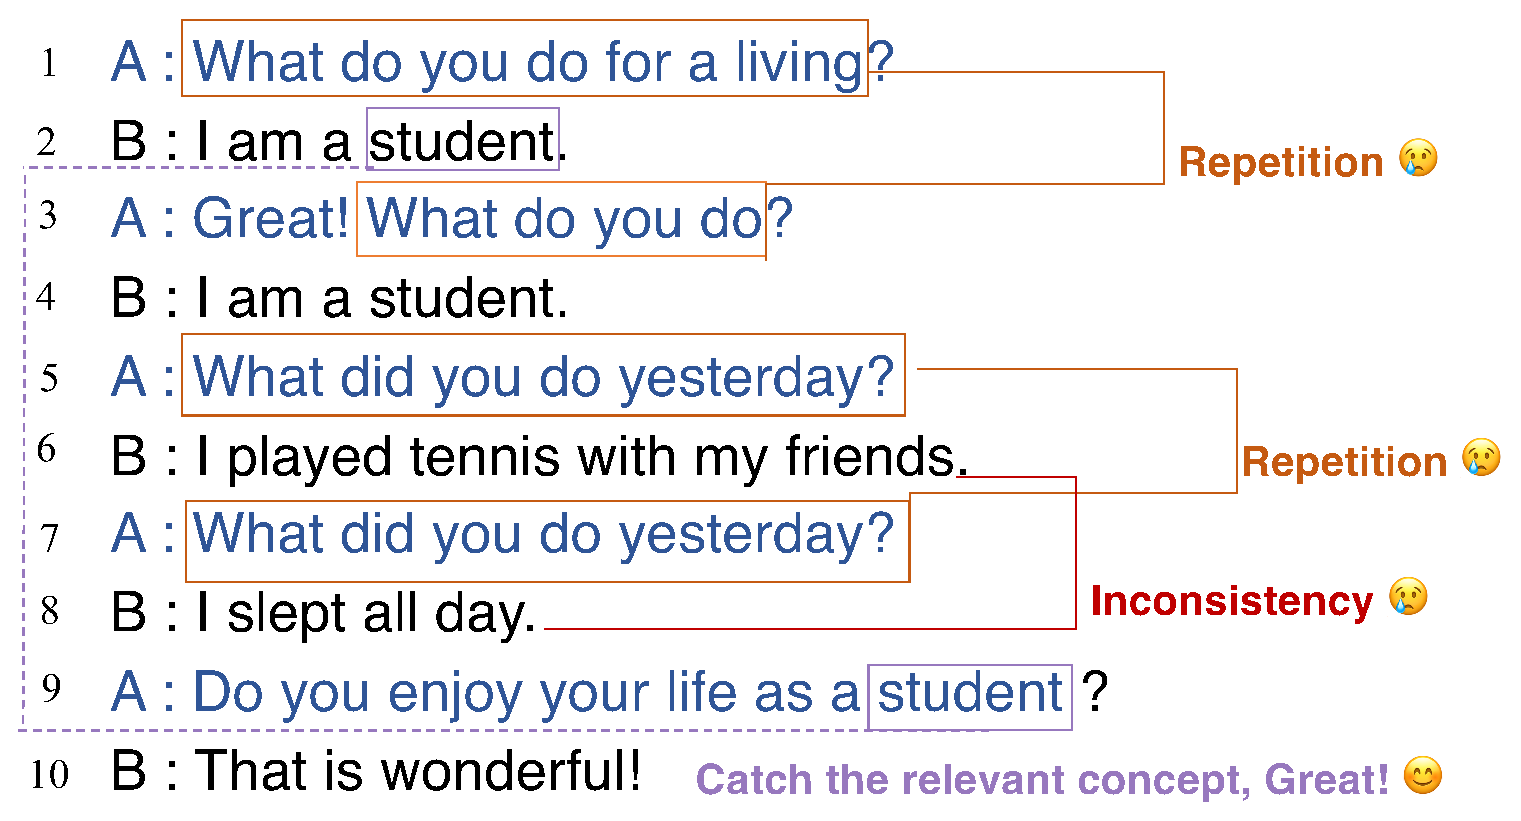
\includegraphics[width=0.95\columnwidth]{example2.eps}
        \caption{A chat snippet between two bots.}
        \label{fig:example}
\end{figure}

Fluency, Knowledge, Proactivity and Specificity are scored for each turn separately
and aggregated at the end of the conversation.
Detection for diversity, consistency and relevance are more involved and are explained
using \figref{fig:example}. 

As for diversity, at each turn $t$, we first check if there exists any repetitive question.  
We can easily find turn 3 and turn 7 repeated turn 1 and turn 5 
respectively. They will then be penalized one point for repetition. 
Repetition is not penalized if the previous turn is already 
marked as a repetitive question. For example, in \figref{fig:example}, 
although turn 4 is considered a repetition of turn 2,  
we are not going to penalize it as turn 3 is a repetitive question. 

The detection of inconsistency is always triggered after the detection of repeated questions. 
If the answers to the same questions are different, we will penalize the current turn, 
such as turn 8 in \figref{fig:example}.

We decide a repetition or an inconsistency by calculating the similarity of the two turns. 
We use a similarity function to complete the calculations, which we will 
discuss in \secref{sec:experiment}. The actual diversity and consistency scores
are the negation from the amount of repetition and inconsistency.

Relevance is assessed as a bonus to reward
a bot if it is able to memorize the important relevant concepts that have shown up 
before in the conversation. We sort the concepts that have shown up in 
chat history by their IDF scores. For example, in turn 9, $A$ 
mentions the concept word ``student'' presented by $B$ in turn 2. With this
turn, $A$ will win a bonus point.


The algorithms and notations for computing diviersty, consistency and relevance are included
in \tabref{tab:functions}, \algoref{algo:rep}, \algoref{algo:inconsist}, and \algoref{algo:bonus}. 

\begin{table}[th]
\centering
\small
\begin{tabular}{c|l}
%\hline
\toprule
\textbf{Notation} & \textbf{Description} \\ \midrule
$t$ & Current turn \\
$H(t)$  &  a list of history turns prior to $t$ \\
$Sim(x,y)$ & similarity between two turns $x$ and $y$ \\
$\sigma_r$ & Threshold for detecting repetition \\
$\sigma_c$ & Threshold for detecting consistency \\
$r$ & Weight for repetition \\
$c$ & Weight for inconsistency \\
$b$ & Weight for bonus \\
$d$ & Min distance between consecutive mentions \\
IDF list & List of lemma in chatlog sorted by IDF\\
$p$ & Percentage of important lemmas in IDF list\\
$R(t)$ &  Repetition penalty for turn $t$ \\
$C(t)$ &  Inconsistency penalty for turn $t$ \\ 
$B(t)$ &  Memory bonus for turn $t$ \\
$Rep(t)$ & A list of repeated turns for turn $t$ \\  
\bottomrule
\end{tabular}
\caption{
Functions and variables in algorithms.}
\label{tab:functions}
\end{table}

\begin{algorithm}[th]
\small
\caption{Scoring for Diversity}
\label{algo:rep}
\hspace*{0.02in} {\bf Input:}
 $t$, $H$, $Sim$, $\sigma_{r}$
; \hspace*{0.02in} {\bf Output: } 
 $R$;
\begin{algorithmic}[1]
\State //Starting to detect repetition
\For {$u$ in $H(t)$}
	\If {$Sim(t,u) \geq \sigma_{r}$}
		\State Add $u$ to $Rep(t)$
	\EndIf
\EndFor
    \If{$len(Rep(t))\geq 0$}
        \If{$t$ is a question and We can find a question in $Rep(t)$}
        \State $ R(t) \leftarrow  R(t) + 1$ 
        \Else
        \If {the previous turn of $t$ is not a repetitive question}
        \State $R(t)) \leftarrow R(t) + 1$ 
        \EndIf
        \EndIf
    \EndIf
\end{algorithmic}
\end{algorithm}


\begin{algorithm}[th]
\small
\caption{Scoring for Consistency}
\label{algo:inconsist}
\hspace*{0.02in} {\bf Input:}
$t$, $H$, $Sim$, $\sigma_{c}$
; \hspace*{0.02in} {\bf Output:  } 
 $C$;
\begin{algorithmic}[1]
\State // Inconsistency detection
 \If {previous turn of $p$ is a repetitive question} 
   \If{ the response $res$ to the question repeated by turn $p$ contradicts turn $i$ with $Sim(t, res) \leq \sigma_{c}$ }
    \State $C(t) \leftarrow C(t) + 1$
   \EndIf
  \EndIf
\end{algorithmic}
\end{algorithm}

\begin{algorithm}[th]
\small
\caption{Scoring for Relevance}
\label{algo:bonus}
\hspace*{0.02in} {\bf Input:}
$t$, $p$, $d$
; \hspace*{0.02in} {\bf Output:  } 
$B$;
\begin{algorithmic}[1]
\State // Assessing the ability of catching relevant concepts\\
$B(t) \leftarrow 0$
\For {all tokens $tk$ in current turn $t$}
 \If {$t$ - previous occurrence turn of $tk > d$ and $tk$ in the top $p\%$ of the IDF list of all tokens in the dialogue} 
   \State $B(t) \leftarrow 1$
  \EndIf
 \EndFor
\end{algorithmic}
\end{algorithm}

At the end of each game, each bot gets seven scores, one for each dimension.  
After pairwise comparison on individual dimension, a bot gains one point for win and zero point for a tie or lose.
The final score of each bot is determined by the sum of their individual scores.
%\KZ{Are these scores positive or negative? Comparable between bots?}

\subsubsection*{Match-level Scoring}
%\KZ{Use an equation to compute the final scores?}
One match which consists of two games, each started with a different bot, 
decides winning or losing between two bots.
For match-level scoring, we mimic the scoring rules of soccer tournament. 
For each match, $W$ points for the winner,  
$T$ points for a tie and 
$L$ points for the loser.
The value of $W$, $T$ and $L$ will be discussed in \secref{sec:ablation}. 

%\KZ{At the match level, we need to consider different starting context for the bots? I think we should present a few options for the reader and say that we are limited to these.}

\subsubsection*{Tournament-level Scoring}
%\KZ{Use an equation to compute the final scores?}
We count the points by simply summing up their scores gained in every match. Currently, several bots with the same final rank are tolerated. For future study, it's possible to mimic more detailed rules presented in sports match such as determine their ranking based on their win-loss relationship in the match between them.  
If they are still tied, we could propose an “overtime” for these two bots, one human judge may observe their performance and then make the decision of the game.


\section{Experiments}
\label{sec:eval}

In this section, we first evaluate the quality of our inferred schemas,
then we perform experiments on the task of link prediction and triple classification.
Finally, we discuss and analyze the errors in our system.

\subsection{Experimental Setup}

\textbf{Knowledge bases.}
We use two knowledge bases throughout our experiments: {\bf FB3m} and {\bf FB15k}.
%We use three knowledge bases throughout our experiments:
%FB15k, FB15k-type and FB (full version).
%FB15k \cite{bordes2013translating} is a widely used benchmark dataset in the task of link prediction and triple classification.
FB15k~\cite{bordes2013translating} is a subset of Freebase 
containing 14,951 entities, 1345 predicates, and 483,142 triple facts.
%Triples in FB15k are split into training / validation / testing parts.
%In order to keep a fair comparison,
We use triples from training split as our knowledge base.
%since all evaluating triples come from OpenIE system.
%Note that FB15k doesn't contain IsA relationship, thus we construct
%a new knowledge base called FB15k-type by adding type information
%of all entities into FB15k.
%Besides, we use Freebase dump of June 2015~\cite{freebase:datadumps}
%as the full version of FB.
%We use these two complementary knowledge bases in link prediction task.
%\tabref{tab:fb-size} shows the statistics of these KBs.
Besides, we construct FB3m from the Freebase dump released of June 2015~\cite{freebase:datadumps},
which contains 3 million popular entities and 50 million triple facts (100 times larger than FB15k).
%Compared with the full dump, FB3m is light-weighted but still
%contains the most valuable knowledge.

\noindent
\textbf{Relation datasets.}
We construct three relation datasets for experiments.
The first two datasets, called ``\textbf{PATTY-100}'' and ``\textbf{PATTY$^+$-100}'',
are extracted from PATTY \cite{nakashole2012patty} OpenIE system, each containing
100 natural language relations.
%We select PATTY \cite{nakashole2012patty} as the OpenIE dataset.
%called ``PATTY-100''.
PATTY contains more than 200,000 different natural language relation synsets
with millions of entity pairs extracted from Wikipedia.
Each entity in PATTY is linked to Freebase through a unique Wikipedia page.
PATTY-100 is for experiments related to FB15k, and contains relations with high
support in PATTY such that all the entities can be found in FB15k.
Conversely, PATTY$^+$-100 is for FB3m related experiments.
It is sampled from all of PATTY and may contain more complex and long-tail relations.
On average, each PATTY-100 relation has a support of 180 facts in
FB15k, and each PATTY$^+$-100 relation has a support of 388 facts in FB3m.
%From top 1,000 distinct PATTY relations sorted by the number of
%relation instances where both arguments are linked to FB15k,
%we randomly pick 100 relations for evaluation. %, called ``PATTY-100''.
%On average, each relation in PATTY-100 contains 180 instances linked to FB15k,
Both PATTY datasets are split into training / validation / testing sets (64\% : 16\% : 20\%).
The third dataset, called ``\textbf{FB15k-37}'', consists of 37 popular predicates
in the domains of ``people'', ``location'' and ``sports'', sampled from FB15k.
FB15k-37 is a subset of FB122 \cite{guo2016jointly},
removing predicates with too small testing data,
and each predicate has at least 10 testing triples.
Experiments on FB15k-37 treats our system as a classic KBC system.

%From top 1,000 distinct PATTY relations sorted by the number of
%relation instances, we randomly pick 100 relations for evaluation.
%Each relation contains 180 instances on average, and we split them into
%training / validation / testing sets (64\% : 16\% : 20\%).
%By manual inspecting, 18 relations are considered complex relations,
%and while the remaining relations are classified as ``ordinary'' relations.

%\begin{table}[ht]
%	\small
%	\centering
%	\caption{Statistics of Freebase used in experiments. \KQ{to be updated.}}
%	\begin{tabular}{|c|c|c|c|}
%		%\toprule
%		\hline
%		Dataset				&	FB15k	&	FB15k-type	&	 FB		\\
%        \hline
%		%Ordinary entities	& 50,718,028	& 3,000,000		&		\\
%        %\hline
%        %Mediator entities	& 36,131,437	& 7,301,261		&		\\
%		%\hline
%		Total entities		&	14,951	&	14,951	&	86,849,465	 \\
%		\hline
%		Distinct relations	&	1,345	&	1,345	&	4,932	\\
%        \hline
%		Types 				&	0		&	xxxx	&	2,071	\\
%		\hline
%		IsA relationships	&	0		&	yyyy	&	zzzz	\\
%		\hline
%		Triple facts		&	483,142	&	483,142	& 280,788,583	\\
%		\hline
%	\end{tabular}%
%	\label{tab:fb-size}%
%\end{table}

\noindent
\textbf{State-of-the-art comparisons.}
For embedding techniques, we take TransE \cite{bordes2013translating},
KALE \cite{guo2016jointly}, TEKE \cite{wang2016text} and
HOLE \cite{nickel2015holographic} as our comparisons.
%TransE models the confidence of a triple fact as vector translations on the
%embeddings of the predicate and two entity arguments.
%%TransE models a relationship as operating translations on the embeddings of
%%subject and object entities. \KQ{Change all subject, object into head, tail??}
%KALE and TEKE are two extensions of TransE.
%KALE introduces logical rules as the combination of atom triple facts with logical connectives,
%therefore the model can learn embeddings from both positive triples and rules.
%TEKE enables each relation to own different representations for different subject and object
%entities, by leveraging the rich context information of a triple fact from web text corpus.
%HOLE is a novel compositional embedding model for representing relationships,
%which is based on the circular correlation of entity vectors.
%
For rule induction techniques, we compare with two models:
SFE \cite{gardner2015efficient} and AMIE+ \cite{galarraga2015fast}.
%One traditional model, called Path Ranking Algorithm \cite{lao2011random},
%extracts all possible paths connecting subject and object entities,
%then learns a feature-based model to represent each relation,
%and SFE is an extension of PRA model, by adding extra subgraph features
%from the surrounding of subject and object entities in the knowledge base.
%AMIE+ first searches possible structures, and then calculates the confidence score
%of each structure by a simple counting strategy in positive triple facts
%(without the step of weight learning).
We also considered Coupled PRA model \cite{wang2016knowledge}
as a comparison. However,
because different relations share almost no entity
pairs in PATTY-100,
the model would degenerate into the traditional PRA model
and hence be strictly superseded by SFE.

\noindent
\textbf{Implementation details.}
We evaluate two variants of our approach: Ours-SC (producing schemas with constraints)
and Ours-SK (schemas skeleton only) .
%The only difference between them is whether
%to explore constraints in schema generation (\secref{sec:candgen}).
%Ours-SK only picks skeletons as candidates (without searching for constraints),
%while Ours-SC is allowed to use all candidate schemas.
%We evaluate our approach under several settings.
%In candidate generation step, we compare two settings:
%``use-skeleton-only'' and ``use-whole-schema'', based on
%whether to explore constraints.
%The first specification only extract path candidates without generating
%constraints, while the latter one is free to use all candidate schemas.
%In schema inference step, we compare two strategies ``random walk''
%and ``zero-one'', described in \secref{sec:schema}.
%\KQ{Will update approach part, mentioning these notations.}
For both variants,
%For each specification, we select the size of priority queue in
%in order to observe how the result varies with the number of candidate schemas.
we set the maximum skeleton length $\tau = 3$,
\footnote{
%Our approach works regardless of the skeleton length. However,
We observed that $\tau > 3$ costs significantly more time with no
substantial benefits.}
%$\tau = 3$,
%tune the minimum support ratio $\gamma$ as in \{5\%, 10\%, 15\%, 20\%\},
%the smoothing parameter $\alpha$ in \{1e-6, 1e-5, 1e-4\}
%and the size of priority queue in
%\{1000, 2000, 3000, 4000, 5000\}.
%||||||| .r20267
%$\tau = 3$,
%tune the minimum support $\gamma$ as in \{5\%, 10\%, 15\%, 20\%\},
%the smoothing parameter $\alpha$ in \{1e-6, 1e-5, 1e-4\}
%and the size of priority queue in
%\{1000, 2000, 3000, 4000, 5000\}.
the size of the priority queue to be 5000.
We tune the minimum support $\gamma$ in the range of \{5\%, 10\%, 15\%, 20\%\},
the smoothing parameter $\alpha$ in \{1e-6, 1e-5, 1e-4\}
and the learning rate in \{0.02, 0.05, 0.1\} on the validation set.
%\KZ{Shall we also eval the effect of different $\tau$? To justify
%why 3 is the right choice.}
%\KQ{Added a footnote here.}
For comparison, we use the existing code for
AMIE+ \footnote{https://www.mpi-inf.mpg.de/departments/databases-and-information-systems/research/yago-naga/amie/},
and SFE system provided by Gardner et al.~\shortcite{gardner2015efficient}
\footnote{https://github.com/matt-gardner/pra},
KALE system by Guo et al.~\shortcite{guo2016jointly},
HOLE and TransE by Nickel et al.~\shortcite{nickel2015holographic}
\footnote{https://github.com/mnick/scikit-kge},
and implement TEKE system by ourselves based on TransE.
All the embedding systems adopt the max-margin model during the learning step.
For KALE, we tune the learning rate in \{0.02, 0.05, 0.1\} and the margin
in \{0.1, 0.12, 0.15, 0.2\}.
For TransE, TEKE and HOLE, we tune the learning rate in \{0.05, 0.1, 0.2\} and the margin
in \{0.5, 1.0, 1.5, 2.0, 2.5\}.


%TODO: Add detail about the other state-of-the-arts.

\subsection{Schema Quality Evaluation}

In this experiment, we focus on how the explicit semantic structure bridges
the gap between Freebase and PATTY$^+$-100 relations.
We compare the top schemas (a.k.a. rules)
of 4 selected example relations produced by Ours-SC, Ours-SK, AMIE+ and SFE,
all of which considered rule induction methods.
The experiment is performed on FB3m, so that each model
can find more different structures.
For each relation from PATTY$^+$-100, we rank the
candidate schemas from Ours-SC and Ours-SK by the learned probability distribution,
while SFE ranks the path features by their feature weights,
and AMIE+ ranks all the rules by their confidence score,
which is the precision of the rule over triple facts in training data.
%Due to many specific rules with the same and highest confidence = $1.0$ in AMIE+,
%we manually pick the most appropriate rule from them.

\figref{fig:relation-example} shows the comparison.
We can learn from examples that:
1) The constraint edges help create more precise semantics.
   Compared with Ours-SK, the schema-based approach learns almost the perfect
   schemas on each example.
2) The quality of top structures from AMIE+ and SFE is not as good as our results.
   AMIE+ ranks rules by confidence and hence prefers more specific rules.
   Once the search depth is increased to 4 or more, the system
   uses huge amount of memory and doesn't return.
   %That's because AMIE+ lacks a tradeoff step, thus top rules always have a high precision
   %but low recall.
   %, therefore we could find rules with necessary constraints  .ranking by confid
   In SFE, the wildcard edge brings about a large amount of flexible path features,
   but most of them don't have clear semantics, and hard to construe by human.


\begin{figure*}[t]
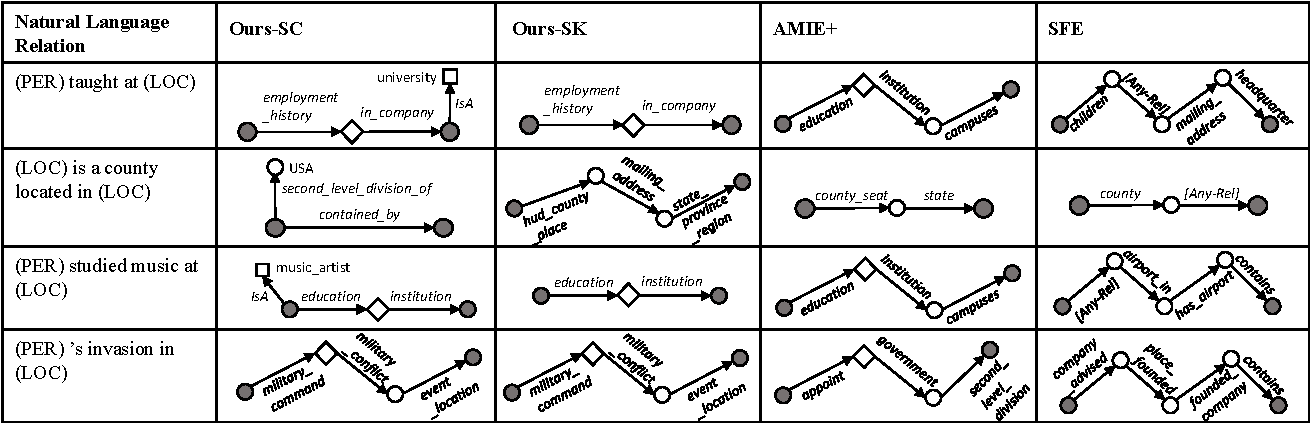
\epsfig{file=case-crop.eps, width=2\columnwidth}
\centering
\caption{Top schemas produced by four systems on 4 complex relations.
%We list top-3 schemas along with probabilities for each relation.
Circle node indicates entities or variables, the two black circles represents
$x_{subj}$ and $x_{obj}$ respectively. Square node represents a type
and diamond node represents a mediator (an n-ary predicate).}
\label{fig:relation-example}
\end{figure*}



As a complementary evaluation, we perform a human judge experiment
on the quality of top ranked schemas produced by Ours-SC and Ours-SK.
%3 annotators, who are familiar with Freebase structure,
%are required to label top 5 schemas of each relation
The evaluators are 3 non-author annotators who are familiar with Freebase.
For each relation, up to top 5 schemas with a probability larger than 0.05 is
labeled with a score in \{0, 0.5, 1\},
indicating ``irrelevant schema'' (semantic drift on the skeleton),
``partial match'' (the skeleton makes sense, but constraints can be improved) and
``perfect match'' (both skeleton and constraints are suitable), respectively.
We first compute the average score for the top $n$ schemas per relation and annotator,
then average these scores over all relations and all annotators to produce
AvgSc@$n$.
The inter-annotator agreement is 0.541 by Kappa coefficient.
As shown in \tabref{tab:average-score}, the schema-based approach
improves the result by up to 13\%.

\begin{table}[t]
	\small
	\centering
	\caption{AvgSc@$n$ results on top-ranked schemas.}
	\label{tab:average-score}
	\begin{tabular}{c|ccc}
						&	n=1		&	n=3		&	n=5			\\
		\hline
		Ours-SK			&	0.44	&	0.37	&	0.34		\\
		Ours-SC			&	\textbf{0.47}	&	\textbf{0.40}	&	\textbf{0.38}
	\end{tabular}
\end{table}


\subsection{Link Prediction}
This task is to predict the missing object in the triple ($e_{subj}$, $r$, $?$),
or the missing subject in ($?$, $r$, $e_{obj}$).
Following the evaluation protocol of KALE \cite{guo2016jointly},
for each triple ($e_{subj}$, $r$, $e_{obj}$) in testing set,
we replace $e_{obj}$ by any other entities $e'_{obj}$ in the knowledge base,
forming a list of wrong triples ($e_{subj}$, $r$, $e'_{obj}$), with only one
positive triple in it.
By using \eqnref{eqn:score-def}, we calculate the score of each prediction in the list
and rank them in descending order,
returning the rank of the correct $e_{obj}$ among all other wrong entities.
Similarly, we can get the rank of $e_{subj}$ at the subject side.
To be consistent with the state-of-the-art systems, we aggregate over all testing triples,
reporting the mean reciprocal rank (MRR)
%, the median value of the ranks (MED),
and the proportion of ranks no larger than $n$ (Hits@$n$, or H@$n$ for short).
%Note that a \textit{lower} MED value indicates a better model.
For each setting, we tune all the parameters based on the MRR score on the validation set.
%\KZ{What about macro F1?}
%\KQ{Nothing to do with F1 in link prediction task, it's in triple classification.
%However, we didn't get a perfect win in F1 metrics, and other papers didn't report F1 also.
%So didn't we.}

Due to the existence of one-to-many relations, some wrong triples ($e_{subj}$, $r$, $e'_{obj}$)
are actually correct and already observed
in the dataset (either in training, validation or testing).
In this case, we follow TransE \cite{bordes2013translating}
and create two settings called ``raw'' and ``filtered''.
In the filtered setting, we remove such correct triples from the triple list
before calculating the rank of each prediction.
Conversely, in the raw setting, we don't remove any triples.


%
%We perform the evaluation on FB15k under filtered setting \KZ{What is this
%setting? Never mentioned before?}.
%\figref{fig:trend-with-budget} shows how the MRR results
%\KQ{on validation set}, vary with the number of candidate schemas.
%From the results, we observe that:
%1) The MRR result increases with the number of candidate schemas in
%every setting, which indicates that larger number of candidates
%leads to a better model.
%2) Compare with strategies on candidate generation, use-whole-schema
%outperforms use-skeleton-only, demonstrating the capability of constraints
%to represent natural language relations.
%3) \KQ{random walk v.s. zero-one, need to get real results before the analysis.}
%
%%\KQ{Figure to be plotted: budget 1k~5k  *  4 different specifications.}
%\begin{figure}[th]
%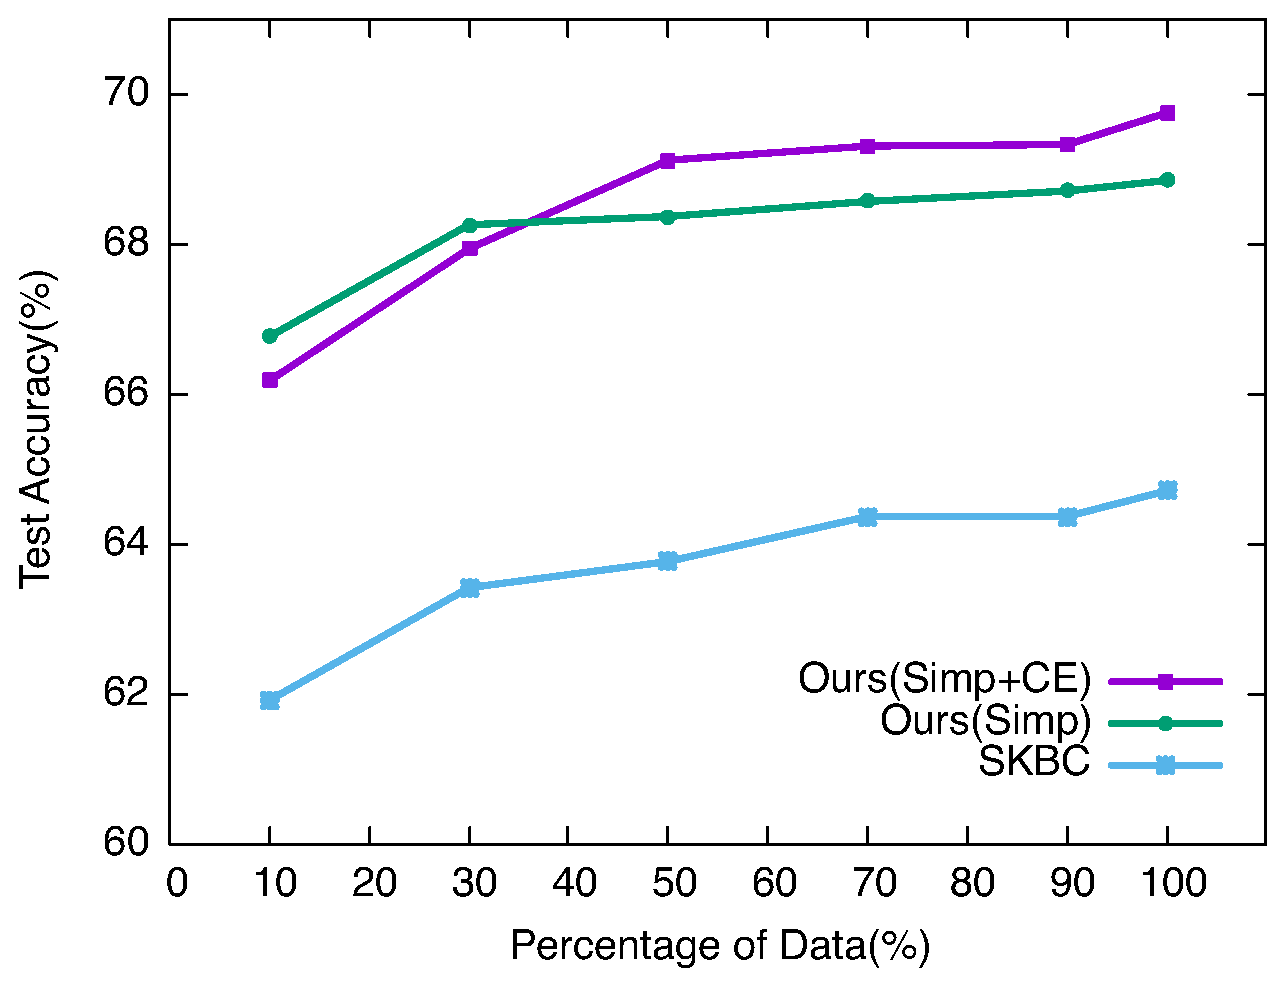
\epsfig{file=trend.eps, width=0.65\columnwidth}
%\centering
%\caption{
%	The trend of link prediction results on FB15k (filtered setting).
%	X axis: size of priority queue,
%	Y axis: MRR score. \KQ{content to be updated.}
%}
%\label{fig:trend-with-budget}
%\end{figure}

%We first evaluate our approach and state-of-the-art systems on PATTY-100 relations.
%Then we compare our approach with state-of-the-art models.
%\KQ{Need to say a little bit about the parameters we used here.}
%\tabref{tab:link-pred-patty} %and \tabref{tab:link-pred-filtered}
%shows the link prediction results on FB15k.

%\KZ{Due to memory issues of the code, SFE method failed to produce any result.
%This is a bit strange: you pick SFE as a comparison but it doesn't work for
%link prediction at all! Better fix this!}
%As we can see, our approach outperforms both embedding and
%other rule induction models.



We perform link predication on FB15k in order to compare with embedding models.
In the following experiments, we use $\gamma=10\%$, $\alpha=1e-4$ and learning rate = 0.1
as the best parameters to achieve the highest filtered MRR score
on the validation set of PATTY-100.
\tabref{tab:link-pred-patty} and \tabref{tab:link-pred-fb15k} shows
the results for PATTY-100 and FB15k-37 respectively.
SFE ran out of memory for both data sets because it needs to enumerate all
possible entities in the KB, and hence is excluded from the tables.
For PATTY-100 relations, our schema based approach outperforms
both embedding and other rule induction models.
Meanwhile, for FB15k-37 predicates, Ours-SK shows nearly the same performance as Ours-SC.
That's because predicates in FB15k-37 may have an equivalent form in KB,
for example, $location.location.containedby \rightarrow !location.location.contains$,
where ``$!$'' indicates the reverse of a predicate, therefore skeletons are precise
enough to represent such predicates.
Furthermore, link predication results on natural language relations are relatively lower
than those on KB predicates.
%Comparing the results on different set of relations,
%the improvements on complex relations are much more significant than those
%on ordinary relations, indicating the usefulness of the extra constraints
%in representing complex relations.
%Besides, the link prediction results on natural language relations
%are relatively lower than
%those results evaluated on FB15k relations \cite{guo2016jointly}.
Two possible reasons are:
1) Each predicate in FB15k-37 has up to thousands of supported instances in FB15k,
while a natural language relation from PATTY-100 only has about 115 training instances.
2) Natural language relations are semantically more ambiguous than KB predicates,
therefore triple facts of different semantics may be mixed during information extraction.
On the other hand, knowledge bases are carefully curated and contain less ambiguity.

\begin{table}[b]
	\small
	\centering
	\caption{Link prediction results on PATTY-100 relations.}
	\label{tab:link-pred-patty}
	\begin{tabular}{|c|ccc|ccc|}
		\hline
				&	\multicolumn{3}{c|}{Raw}
				&	\multicolumn{3}{c|}{Filtered}	\\
		\cline{2-7}	
				&	MRR	&	H@3	&	H@10
				&	MRR	&	H@3	&	H@10		\\
		\hline
		TransE
				&	0.112	&	12.4	&	27.1
				&	0.129	&	14.5	&	29.9	\\	%m1.75_lr0.10
		KALE
				&	0.112	&	12.5	&	25.4
				&	0.125	&	14.4	&	27.5	\\	%Test-base-k100-d0.15-ge0.02-gr10-filt.eval_KQ
		TEKE
				&	0.101	&	10.9	&	24.1
				&	0.114	&	12.6	&	26.3	\\
		HOLE
				&	0.109	&	10.5	&	23.3
				&	0.121	& 	12.3	&	25.8	\\	%log.hole_d100_m0.25_lr0.05
		%AMIE+
		%		&	0.119	&	23.5
		%		&	0.132	&	24.4	\\
		AMIE+
				&	0.148	&	16.5	&	29.3
				&	0.174	&	19.5	&	\textbf{31.9}	\\
		\hline
		Ours-SK
				&	0.169	&	18.2	&	29.3
				&	0.179	&	19.1	&	30.4	\\		%Blackhole
		Ours-SC
				&	\textbf{0.172}		&	\textbf{18.5}	&	\textbf{29.8}
				&	\textbf{0.185}		&	\textbf{19.9}	&	31.5	\\	%Blackhole
		\hline
	\end{tabular}
\end{table}

%\begin{table*}[ht]
%	\small
%	\centering
%	\caption{Link prediction results on FB15k (raw setting).}
%	\begin{tabular}{|c|ccccc|ccccc|ccccc|}
%		%\toprule
%		\hline
%				&	\multicolumn{5}{c|}{Complex relations}
%				&	\multicolumn{5}{c|}{Ordinary relations}
%				&	\multicolumn{5}{c|}{Overall}	\\
%		\cline{2-16}	
%		\multirow{2}{*}{}	&	\multirow{2}{*}{MRR}	&	\multirow{2}{*}{MED}	&	\multicolumn{3}{c|}{Hit@n(\%)}
%							&	\multirow{2}{*}{MRR}	&	\multirow{2}{*}{MED}	&	\multicolumn{3}{c|}{Hit@n(\%)}
%							&	\multirow{2}{*}{MRR}	&	\multirow{2}{*}{MED}	&	\multicolumn{3}{c|}{Hit@n(\%)}	\\
%				&	&	&	3	&	5	&	10	
%				&	&	&	3	&	5	&	10	
%				&	&	&	3	&	5	&	10	\\
%		\hline
%		TransE
%				&	0.089	&	75.0	&	11.7	&	17.2	&	23.2
%				&	0.081	&	66.0	&	 8.1	&	12.1	&	19.6
%				&	0.082	&	68.0	&	 8.9	&	13.2	&	20.4	\\
%		KALE	
%				&	0.142	&	47.0	&	17.5	&	23.4	&	30.5
%				&	0.104	&	42.0	&	11.2	&	16.0	&	24.0
%				&	0.112	&	\textbf{43.0}	&	12.5	&	17.6	&	25.4	\\
%		TEKE	
%				&	0.119	&	68.4	&	14.7	&	19.5	&	27.6
%				&	0.096	&	57.2	&	9.8  	&	14.6	&	23.1
%				&	0.101	&	59.0	&	10.9	&	15.7	&	24.1	\\
%		HOLE
%				&	0.153	&	55.0	&	16.0	&	20.5	&	27.4
%				&	0.097	&	51.0	&	 9.1	&	13.9	&	22.2
%				&	0.109	&	52.0	&	10.5	&	15.4	&	23.3	\\
%		%\hline
%		%SFE-AnyRel
%		%SFE-OneSide
%		AMIE+
%				&	0.164	&	76.3	&	18.2	&	21.9	&	26.6
%				&	0.107	&	68.3	&	11.3	&	15.8	&	22.6
%				&	0.119	&	69.5	&	12.7	&	17.1	&	23.5	\\
%		Ours
%				&	0.225	&	42.5	&	24.3	&	27.8	&	34.7
%				&	0.158	&	43.0	&	16.9	&	21.0	&	28.5
%				&	\textbf{0.172}	&	\textbf{43.0}	&	\textbf{18.5}	&	\textbf{22.5}	&	\textbf{29.8}	\\
%		\hline
%	\end{tabular}
%	\label{tab:link-pred-raw}
%\end{table*}

\begin{table}[tbh]
	\small
	\centering
	\caption{Link prediction results on FB15k-37 relations.}
	\label{tab:link-pred-fb15k}
	\begin{tabular}{|c|ccc|ccc|}
		\hline
				&	\multicolumn{3}{c|}{Raw}
				&	\multicolumn{3}{c|}{Filtered}	\\
		\cline{2-7}	
				&	MRR	&	H@3	&	H@10
				&	MRR	&	H@3	&	H@10	\\
		\hline
		TransE
				&	0.310			&	39.3	&	53.2
				&	0.394	&	52.5	&	65.0	\\	%log.transe_m2.00_lr0.10.train_lp
		KALE
				&	0.342	&	40.6	&	53.0
				&	0.410	&	48.7	&	60.6	\\	%Test-KALE-1110-k100-d0.12-rd0.12-ge0.05-gr10-w1(0.1)-w2(1)-w3(0)-w4(0)-filt.eval_KQ
		TEKE
				&	0.288	&	35.7	&	49.2
				&	0.339	&	43.0	&	56.5	\\
		HOLE
				&	0.234	&	26.7	&	39.5
				&	0.323	& 	36.5	&	50.5	\\	%log.hole_m0.25_lr0.10.train_lp
		AMIE+
				&	0.395	&	46.1	&	53.7
				&	0.562	&	60.0	&	68.9	\\
		\hline
		Ours-SK
				&	0.425	&	47.8	&	55.6
				&	0.664	&	68.8	&	73.0	\\		%Darkstar
		Ours-SC
				&	\textbf{0.427}		&	\textbf{48.1}	&	\textbf{55.7}
				&	\textbf{0.671}		&	\textbf{69.3}	&	\textbf{73.3}	\\		%Darkstar
		\hline
	\end{tabular}
\end{table}

%\begin{table*}[ht]
%	\small
%	\centering
%	\caption{Link prediction results on FB15k (filtered setting).}
%	\begin{tabular}{|c|ccccc|ccccc|ccccc|}
%		%\toprule
%		\hline
%				&	\multicolumn{5}{c|}{Complex relations}
%				&	\multicolumn{5}{c|}{Ordinary relations}
%				&	\multicolumn{5}{c|}{Overall}	\\
%		\cline{2-16}	
%		\multirow{2}{*}{}	&	\multirow{2}{*}{MRR}	&	\multirow{2}{*}{MED}	&	\multicolumn{3}{c|}{Hit@n(\%)}
%							&	\multirow{2}{*}{MRR}	&	\multirow{2}{*}{MED}	&	\multicolumn{3}{c|}{Hit@n(\%)}
%							&	\multirow{2}{*}{MRR}	&	\multirow{2}{*}{MED}	&	\multicolumn{3}{c|}{Hit@n(\%)}	\\
%				&	&	&	3	&	5	&	10	
%				&	&	&	3	&	5	&	10	
%				&	&	&	3	&	5	&	10	\\
%		\hline
%		TransE
%				&	0.097	&	69.0	&	13.0	&	18.7	&	25.0
%				&	0.092	&	62.0	&	 9.7	&	14.2	&	22.2
%				&	0.094	&	63.0	&	10.4	&	15.2	&	22.8	\\
%		KALE	
%				&	0.153	&	43.0	&	19.9	&	25.5	&	32.5
%				&	0.118	&	39.0	&	12.9	&	18.0	&	26.1
%				&	0.125	&	\textbf{39.0}	&	14.4	&	19.6	&	27.5	\\
%		TEKE	
%				&	0.129	&	64.3	&	16.2	&	21.4	&	29.1
%				&	0.109	&	52.7	&	11.7	&	16.9	&	25.6
%				&	0.114	&	54.0	&	12.6	&	17.9	&	26.3	\\
%		HOLE
%				&	0.162	&	50.5	&	17.4	&	21.8	&	29.0
%				&	0.109	&	47.0	&	10.9	&	16.1	&	24.9
%				&	0.121	&	47.0	&	12.3	&	17.3	&	25.8	\\
%		%\hline
%		%SFE-AnyRel
%		%SFE-OneSide
%		AMIE+
%				&	0.180	&	73.8	&	18.6	&	22.4	&	27.5
%				&	0.120	&	63.5	&	12.5	&	17.0	&	23.6
%				&	0.132	&	65.0	&	13.8	&	18.2	&	24.4	\\
%		Ours
%				&	0.237	&	41.0	&	25.2	&	29.1	&	35.5
%				&	0.171	&	40.0	&	18.4	&	22.4	&	30.5
%				&	\textbf{0.185}	&	40.0	&	\textbf{19.9}	&	\textbf{23.8}	&	\textbf{31.5}	\\
%		\hline
%	\end{tabular}
%	\label{tab:link-pred-filtered}
%\end{table*}





\subsection{Triple Classification}
This task is to predict whether a new triple ($e_1$, $r$, $e_2$) is correct or not.
As a binary classification task, we need to generate negative triples for evaluations.
Following the strategy used in KALE \cite{guo2016jointly},
for each positive triple in the validation and test set,
we generate 10 negative triples by randomly corrupting the entities, 5 at the subject
position and 5 at the object position. We ensure that each corrupted entity
has appeared in some other positive triples at the same position,
and all corrupted triples do not exist in either the training, validation or testing set.

For each relation, we rank all positive and negative triples
by their likelihood values (see \eqnref{eqn:likelihood-def})
in descending order, and calculate the average precision.
We report the mean average precision (MAP) aggregated over all relations.
We perform the experiment on FB15k, and \tabref{tab:triple-clsf} shows the result on
different relation datasets.

Our system outperforms the other baseline methods on the PATTY-100 dataset,
however, Ours-SK beats Ours-SC, because the negative triples cannot 
be distinguished by the constraints, hence the SC approach has no advantage.
For example, instead of generating a child's own mother as a negative example,
we generate the father of a random child. 
%(what we generated in the current experimental setting)
%as negative data makes the classification problem harder, and shows the value of constraints.
%While in link prediction, the constraints play an important role to 
%rank positive entities higher.
%Moreover, we find that there's almost no difference
%between our two variances on FB15k-37, that's not unexpected because skeletons
%are enough to represent the majority of these predicates.


%Observing results of each model, it's interesting to find that all rule induction models
%performs much better than embedding techniques, which reveals us that
%explicit semantic feature mining could help to find more precise representations,
%especially when the training data is small.
%Ours-SC outperforms the other embedding methods on PATTY-100 dataset, demonstrating the
%importance of constraints. However, the gap could be bigger if the negative triples
%are generated to distinguish the constraints, e.g., for father-of relation,
%using a child's own mother instead of a random father or a random mother as negative data.

\begin{table}[tbh]
	\small
	\centering
	\caption{MAP results on triple classification task.}
	\begin{tabular}{|c|cc|}
		%\toprule
		\hline
							& PATTY-100	&	FB15k-37 	\\
        \hline
		TransE				&	0.304	&	0.666	\\	% m0.25, lr0.05	|	m1.00, lr0.10
		KALE				&	0.309	&	0.654	\\
		TEKE				&	0.282	&	0.631	\\
		HOLE				&	0.308	&	0.680	\\	% m0.25, lr0.20	|	m0.20, lr0.10
		SFE					&	0.329	&	0.621	\\	% due to data shrinking ...
		AMIE+				&	0.226	&	0.730	\\	
		\hline
		Ours-SK				&	\textbf{0.408}	&	\textbf{0.804}	\\	
		Ours-SC				&	0.403	&	0.803	\\
		\hline
	\end{tabular}
	\label{tab:triple-clsf}
\end{table}



\subsection{Error Analysis}

%\figref{fig:relation-example} shows the paraphrasing results of
%selected relations.
%Show a case-by-case P/R/F1/RR?
%The results of top-ranked schemas show us that our paraphrasing system
%is able to produce concrete and precise structural representations.
Our system may fail to capture the correct semantics in some natural language relations.
We have analyzed the results in the above experiments and
found several main causes of error.

1. Relation instances extracted by Open IE system could be incorrect.
%PATTY extracts relation instances by mining the dependency path in a sentence,
%which may lead to wrong arguments.
For example, given the relation \textit{``served as''}, PATTY extracted
an incorrect entity pair (William Dennison Jr., Ohio) from the sentence
\textit{``Dennison served as the 24th Governor of Ohio and as U.S. Postmaster General ...''},
while the correct object should be ``Governor of Ohio''.

2. PATTY relation synset mixed semantically different but lexically similar
relation patterns, bringing ambiguity in the relation.
For example, in PATTY's \textit{``'s wife''} relation synset, we found a small list of instances
where the object is actually husband, due to an opposite pattern \textit{``the wife of''}.
This phenomenon prevents us from finding correct gender constraints.
%These instances are due to another pattern in the synset,
%\textit{``the wife of''}, which gives the exact opposite semantics.
%though our system is able to filter out noisy instances, the learned schema
%distribution would be affected if the percentage of noisy data is large.

3. Knowledge base lacks necessary information for representing certain relations.
Freebase doesn't hold knowledge about trivial relations like \textit{``talk to''},
even for non-trivial relations, required predicates could be missing in Freebase.
Given the relation \textit{``(singer) performed in (LOC)''}, FB contains			% synset 0246
neither \textit{place\_visited} nor \textit{hold\_concerts\_in} predicate, therefore
it's hard to summarize into a precise representation.

4. Sometimes a meaningful schema is filtered out due to
the search space limits in candidate searching step.
In relation \textit{``(actor) starring with (actor)''},
the length of the most suitable skeleton
\footnote{The skeleton is $actor \rightarrow med. \rightarrow film \rightarrow med. \rightarrow actor$.}
is 4, hence the system failed to discover it under restriction $\tau$ = 3.

%\KZ{This is why I said we should evaluate the impact of $\tau$.}
%
%\KZ{After reading this paper, one thing that puzzles me is that why is this
%method called paraphrasing natural language relations to knowledge base? The
%approach you are proposing can be used for ordinary KB completion task, right?
%In other words we are not making use of the natural language feature at all.
%I think perhaps we can include some experiments you did with NL features to
%show that NL features are not necessary and explain why. This will clear the
%doubt of some readers.}


%\section{Experiments}
\label{sec:experiments}
In this section, we conduct
extensive experiments on slogan generation 
to evaluate the performance
of the proposed model SALE.
We introduce the dataset, 
the competing models and parameter settings,
as well as the evaluation metrics.
We also demonstrate the experimental results in a series of evaluations
and perform further analyses on the effectiveness of our approach
in generating accurate, fluent, informative and attractive slogans.

\subsection{Dataset}
\label{sec:dataset}
We first introduce the text corpora we create
for slogan generation task in e-commerce.
Then we describe the evaluation dataset we used in
our following experiments.
The datasets are released at \url{https://202.120.38.146/slogan/}.

\subsubsection{Dataset for Slogan Generation}
\label{sec:corpora}
%In this section, we describe the experimental setup,
%especially the hyper-parameter configurations of 
%the Seq2Seq framework we used in following experiments. 
%We also detail dataset used in our experiments.
Slogan generation in E-commerce is a relative new problem.
Thus, there is a lack of dataset for this task.
We created a new dataset, containing 
the basic information of the topics attending to potential focuses or selling-points,
including the topic and its item preference, as well as the slogan.
The data are collected from Taobao, a large-scale website for e-commerce in China.

We use the pattern of ``\emph{PV} + \emph{CG}" 
to construct topics from frequent phrases mining from largely amount
of query logs and product titles.
The product titles are composed by the sellers and content producers on the
website.
We construct multiple item preferences for each topic by sampling items from 
secondary categories as well as human intervention to 
make the items with an item preference concentrate more on a specific focus 
or selling-point.
Thus, in each instance, a topic is annotated with an item preference semi-automatically
by leveraging the category ontology introduced in \secref{sec:introduction}.
Then, we recruit experts to write a slogan for each data instance.
Overall, the dataset contains 857 topics and 
in total 3,555 $(x, p, y)$ instances after preprocessing.

We use four splits named (train/dev/LMdev/test) in our experiments.
Note that, the LMdev split is for 
hyper-parameter $\beta$ tuning (see \secref{sec:shallow_fusion} in details).
The splits are randomly divided based on topics 
proportionally by 90\%, 5\%, 1.5\% and 3.5\%.
Thus each split of (train/dev/LMdev/test) includes 771, 43, 13, 30 topics separately,
and correspond to 3132 training instances, 231 development instances, 
50 LM development instances, as well as 142 test instances.

%For the evaluation dataset, 
\subsubsection{Evaluation Dataset}
\label{sec:eval_dataset}
We perform algorithm evaluation and human evaluation
in our experiments (see \secref{sec:metrics} in details).
Thus we provide two evaluation datasets separately for each.
We directly use all the 142 instances of test split in \secref{sec:corpora},
referred as FULLtest,
for the algorithm evaluation which are based on automatic scoring systems,
such as BLEU.
Besides, we randomly sample 50 instances from the test split
to form a small evaluation dataset for human evaluation,
referred as HUMtest.


\subsection{Compared Methods}
\label{sec:compared}
In this section, we introduce the baseline and choices for 
our model components, as well as the parameter settings
used in those models.

\subsubsection{Baselines and SALE}
\label{sec:baselines}
According to the problem statement (in \secref{sec:problem})
and the proposed item preference fusion methods (in \secref{sec:preference}),
the models for comparison backed by Seq2Seq framework are mainly one-way input models and two-way input models.

One-way input models (prefixed by \emph{One}) takes in one-way input as the source sequence,
and the slogan as its target sequence, without considering 
semantics enhancement or incorporating pretrained language model.
There are three one-way input baselines with different inputs.
\textbf{One-T} (\textbf{t}opic) model
takes the topic itself as its source sequence,
while \textbf{One-P} (item \textbf{p}reference) model takes
the titles of items as its source sequence.
Then, 
%while 
\textbf{One-CAT} (con\textbf{cat}nating) model 
concatenates the topic and its item preference with special token \emph{SEP}
as a separator, and takes the sequence of concatenation as its source sequence.

The two-way input models (prefixed by \emph{Two})
are designed to treat topics and item preferences heterogeneously.
We propose two kinds of two-way input models
based on different heterogeneous inputs fusion methods 
(see details in~\secref{sec:preference}).
%we propose two fusion methods in \secref{sec:preference}
%to combine the heterogeneous inputs.
\textbf{Two-BiAttn} (\textbf{bi}directional \textbf{att}ending) model use the two-way bidirectional attending
to combine the representations of topics and that of item preferences.
\textbf{Two-CAT} (con\textbf{cat}nating) model use two-way concatenating strategy 
to fuse the heterogeneous outputs of encoders.

For \textbf{SALE}, 
we incorporate the semantics enhancement module
(in \secref{sec:semantics}) to enrich
the deep contextualized representations
backed by Two-CAT baseline.
\textbf{SALE+PLM} integrates
%On the basis of SALE, 
%we integrate
pre-trained language model (PLM) 
into SALE at inference time in order to improve
the generalization and robustness of the model.
%Specially, SALE identifies the \emph{is-a} relations
%among heterogeneous inputs and
%increase the semantic capacity of the model for better contextualized representations
%knowledge-aware module

\subsubsection{Parameter Settings}
We use an architecture of 8 stacked convolutional layers 
for both the topic encoder and the item preference encoder
as well as the decoder parts with kernel width as 3.
To enable deep convolutional networks, 
we add residual connections~\cite{he2016deep} from the input of each convolution
to the output of the layer as well.
For each convolutional layer, we set the hidden vector size as 512
and the embedding size as 256.
To alleviate the overfitting problem, we add the dropout ($p=0.2$)
layer~\cite{srivastava2014dropout} for all convolutional layers and fully connected layers.

To optimize the proposed models,
we use Nesterov's accelerated gradient method
~\cite{sutskever2013importance} with gradient clipping 0.1
~\cite{pascanu2013difficulty},
momentum 0.99, and 
learning rate 0.2.
We terminate the training process when the learning rate drops 
below 10e-5.
We set beam size as 5 for the beam search algorithm
in the testing step.
The hyper-parameter $\beta$ of SALE-PLM (in ~\eqnref{eq:shallow_fusion})
was selected to maximize the generation performance
on the LMdev split by grid search, from the range 1e-4 and 0.1.


\subsection{Evaluation Metrics}
\label{sec:metrics}
We perform both algorithm evaluation and human evaluation
in our experiments.
Specially, we evaluate our model on generation quality which includes
the automatic scoring metrics such as
BLEU and lexical diversity,
as well as a number of human-evaluation metrics.

\paragraph{BLEU}
The BLEU algorithm~\cite{papineni2002bleu} compares consecutive phrases of the 
generated slogan with the consecutive phrases it finds
in the reference slogan, and counts the number of matches, in a weighted fashion.
A higher BLEU score indicates a higher degree of similarity with the reference
slogan.
We compare all competing models on test split in terms of the BLEU score as a sanity check.
We also use BLEU score as the standard metric to finetune
hyper-parameter $\beta$ in SALE+PLM model.

\paragraph{Lexical Diversity}
A common problem in automatic text generation is that the system tends to generate safe
answers with enough diversity~\cite{li2016deep}.
A low diversity score often means generated contents are general and vague, 
while higher diversity means the generated contents are more informative and 
interesting.
Following~\cite{ChenLZYZ019}, we calculate the number of distinct n-grams produced on the test split
as the measurement of the diversity of generated descriptions.

\paragraph{Human-evaluation Metrics}
Automatic scoring metrics including BLEU score and lexical diversity are competitive and inexpensive to operate.
However, they do not consider
other important aspects such as intelligibility and grammatical correctness (or fluency) of slogan.
We use several human-evaluation metrics
to evaluate competing models on various perspectives.
\begin{itemize}
	\item \textbf{Overall quality} is designed to measure the
	overall generation quality of model.
	\item \textbf{Relevancy} is used to measure the content relevancy of generated slogan to the given topic and items.
	\item \textbf{Fluency} focus on the intelligibility and grammatical correctness of generated slogan.
	\item \textbf{Interestingness} takes personification and attractiveness into account.
\end{itemize}


\subsection{Performance Comparisons and Analysis}
\label{sec:results}


In this section, we conduct an analysis of our proposed model
to evaluate the contribution of item preference fusion module and
semantics enhancement module as well as the integration of 
pre-trained language model.

We evaluate competing models on FULLtest and HUMtest 
as we described in \secref{sec:eval_dataset}.
The comparison results of slogan generation are shown in 
\tabref{tab:auto_eval} and \tabref{tab:human_eval}.
For human evaluation, we recruit three experts as annotators 
and ask them to give scores on each aspect of generated slogan, 
range from 1 to 5,
then average the scores of each aspect on HUMtest as 
human evaluation results.


\begin{table*}[th]
	%	\small
	\centering
	\caption{Slogan generation results comparison with baseline methods using FULLtest.}
	\label{tab:auto_eval}
	\begin{tabular}{lcccc}
		\hline
		Model %& Overall quality 
		& BLEU &  Diversity (n=2) ($\times 10^2$ )& Diversity (n=3) ($\times 10^2$ ) & Diversity (n=4) ($\times 10^2$ ) \\
		\hline
		One-T %&  3.30  
		&  28.34 &  2.25   &  2.45  &  2.37 \\
		One-P %&  3.86  
		&  41.11 &   4.74 &    5.99 & 6.33 \\
		One-CAT  % & 3.82  
		& 38.86  &  3.86 &  4.77  & 4.94 \\
		Two-BiAttn  % & 3.86  
		& 36.99  &  4.82 &  5.87  &  6.03   \\
		Two-CAT % & 3.95
		& 40.59  &  4.89 &  5.99  &  6.22 \\
		\hline\hline
		SALE % & \textbf{4.16}  
		& 42.31  & 4.87  &  6.20 &  6.55  \\
		SALE+PLM % & -  
		& \textbf{42.36}   &  \textbf{4.89} & \textbf{6.23}  &  \textbf{6.57}  \\
		%		SingleSG$_{\mathrm{concept}}$ & 28.34 &  3.30 & 3.32 & 4.31 & 4.38 \\
		%		SingleSG$_{\mathrm{items}}$& 41.11 & 3.84 & 4.0 & 4.30 & 4.22  \\
		%		MultiSG-{biattn} & 36.99 & 3.86 & 4.05 & 4.17 & 4.11 \\
		%		MultiSG-{cat} & 40.59 & 3.95 & 4.13 & 4.34 & 4.23  \\
		\hline 
	\end{tabular}
\end{table*}



\begin{table}[th]
	\small
	\centering
	\caption{Human evaluation for slogan generation task using HUMtest.}
	\label{tab:human_eval}
	\begin{tabular}{lcccc}
		\hline
		Model & Overall quality & Relevancy &  Fluency & Interestingness \\
		\hline
		One-T &  3.30  &  3.32 &  4.31   &  4.38 \\
		One-P &  3.84 &  4.0 &   4.30 &    4.22  \\
		One-CAT  &  3.62  & 3.94  & 4.24  & 4.18  \\
		Two-BiAttn  & 3.86  & 4.05  &  4.16  &  4.11     \\
		Two-CAT & 3.95  & 4.13  &  4.34 &  4.23   \\
		\hline\hline
		SALE & \textbf{4.16}  & \textbf{4.32}  & \textbf{4.53}  &  \textbf{4.43}  \\
		SALE+PLM & -  & -   &  - &   -  \\
		%		SingleSG$_{\mathrm{concept}}$ & 28.34 &  3.30 & 3.32 & 4.31 & 4.38 \\
		%		SingleSG$_{\mathrm{items}}$& 41.11 & 3.84 & 4.0 & 4.30 & 4.22  \\
		%		MultiSG-{biattn} & 36.99 & 3.86 & 4.05 & 4.17 & 4.11 \\
		%		MultiSG-{cat} & 40.59 & 3.95 & 4.13 & 4.34 & 4.23  \\
		\hline 
	\end{tabular}
\end{table}



Firstly, we show the importance of item preference for  slogan generation.
We introduce item preference features for specific topic
using category ontology as discussed in \secref{sec:preference}.
Topic and its item reference are simply concatenate into one input sequence
in One-CAT model. 
As we can see that One-CAT substantially outperforms One-T which only use topic as input
with an advantage of +0.32 overall quality (relatively 9.7\%), +10.5 BLEU, +110.7\% diversity ($n=2$), +144\% diversity ($n=3$) and +81\% diversity ($n=4$),
Thus, item preference plays an important role in slogan generation task.

However, the results show that
One-P model which only takes in item preference as input outperforms
One-CAT on various metrics.
This imposes that topic and item preference are two heterogeneous inputs,
thus we should treat them differently in the model using item preference fusion method.
Next, we analyze the contribution of item preference fusion methods proposed
in \secref{sec:preference}
by comparing One-CAT, Two-BiAttn and Two-CAT.
We can see that show that two-way concatenating method for Two-CAT
substantially outperforms two-way directional attending for Two-BiAttn.
Though Two-CAT model slightly decreases on BLEU compared to One-P,
Two-CAT outperforms One-P according to human evaluation shown in \tabref{tab:human_eval}.
This suggests that two-way bidirectional attending fusion 
makes the semantics corruption between two heterogeneously deep contextualized representations.
Therefore, two-way concatenating fusion method is more effective for 
heterogeneous inputs combination.

Our proposed \emph{is-a} knowledge-aware model SALE 
is backed by Two-CAT, equipping with the semantics enhancement module.
Results show the effectiveness of semantics enhancement module
proposed in \secref{sec:semantics}.
As shown in \tabref{tab:human_eval} and \tabref{tab:auto_eval}, 
SALE outperforms Two-CAT by a substantial margin.
Specially, semantics enhancement improves the
diversity scores ($n=3, 4$) 3.5\%, 5.3\% separately .
SALE also achieves an improvement of 1.72 (relatively 4.24\%) in terms of BLEU, 
as well as an improvement of 0.57 in terms of overall quality.
We can see that SALE outperforms all previous baselines on every aspect.
Thus SALE is able to generate accurate, fluency, informative and attractive slogans.
We further illustrate this in \secref{sec:cases}. 



Lastly, we analyze the contribution of pre-trained language model integration
comparing results of SALE and SALE+PLM.
As shown in \tabref{tab:auto_eval}, 
incorporating PLM at inference stably improves the diversity 
that performs best at every n-gram diversity scores ($n=2,3,4$).
Note that, we finetuned hyper-parameter $\beta$ for SALE+PLM 
in terms of BLEU score on LMdev split,
and SALE+PLM with $\beta = 2e\mathrm{-}4$ achieves best BLEU score as 42.94.
Thus, we use $\beta=2e\mathrm{-}4$ for SALE+PLM model in test.
As shown in \tabref{tab:auto_eval}, SALE+PLM 
outperforms all competing models in terms of BLEU score as 42.36 
on FULLtest dataset.
Since the results generated by SALE and SALE+PLM are nearly the same on HUMtest,
their human evaluation results are same, 
we do not show result of SALE+PLM in \tabref{tab:human_eval}.
We can see that in this case the improvement of PLM integration is minor but stable, 
on both BLEU score and diversity scores.
We argue that such PLM integration makes our model more robust.

% the contribution of item preferences in one-way input models: OneT, OneP, OneCAT
% item preference fusion methods for two-way input models: OneCAT, Two-BiAttn, Two-CAT
% is-a knowledge-aware model SALE: Two-CAT, SALE, SALE+PLM




\subsection{Case Studies}
\label{sec:cases}
In this section, we perform case studies to observe 
how our propose methods influence the generation so that
the model can generate different slogans for a specific topic
according to different item preferences.
Besides, our proposed \emph{is-a} knowledge-aware model SALE generate higher quality slogans
benefiting from semantics enhancement.

%The running example in \tabref{sec:introduction} illustrates 

In \tabref{tab:vary_preference}, % \tabref{tab:vary_preference}
two item preferences are provided for topic ``早教玩具" (early education toys).
The first preference consists of musical toys such as ``音乐拍拍鼓" (musical patting drum),
which focuses on music education for children,
while the second preference is mainly about ``手摇铃" (rattle) which focuses on improving concentration ability 
as well as soothe emotions for babies.
The second example of 
\tabref{tab:vary_preference} is the running example we discussed in \secref{sec:introduction}.
The proposed model SALE successfully captures those focuses 
and generate attractive slogans accordingly.
For example, SALE generates \emph{music enlightenment}
for the focus of musical patting drum
and generates \emph{soothe baby's emotion } for the focus of 
rattle.
As shown in \tabref{tab:vary_preference}, 
we use red color to mark the preferences and its effects for slogan generation.

We also demonstrate the effectiveness of semantics enhancement
by comparing slogans generated by SALE and Two-CAT in \tabref{tab:semantics}.
%as shown in \tabref{tab:semantics}.
\tabref{tab:semantics_a} shows two example topics associated with an item preference each.
The entities involved in \emph{is-a} relations
have been marked as blue. 
The third column of \tabref{tab:semantics_a} demonstrates the 
identified relations.
\tabref{tab:semantics_b} compares slogans generated by SALE and Two-CAT
for the topics in \tabref{tab:semantics_a}.
Results show that SALE enhanced by \emph{is-a} knowledge 
tends to integrate the inferred user needs into slogan,
for example \emph{the first choice when preparing a gift for mom} for ``large size mother-dress"
and \emph{always protect you} for ``outdoor sports protective gear",
which further promotes user interests.


%\KZ{You need to translate these into English.}
% Please add the following required packages to your document preamble:
% \usepackage{multirow}
\begin{table*}[th!]
\begin{center}
\caption{Two examples of generated slogans by the proposed model SALE, varying
	the item preference while fixing the topic as input.}
\label{tab:vary_preference}
\small
%\subfloat[Example of slogans generated by SALE.]{
%	\label{tab:vary_preference_a}
		\begin{tabular}{c|c|c}
		\hline
%		\multicolumn{1}{c}{topic}  
		topic                                                                    
		& item preference                   
%		& semantic relations                                                                                                                    
		& slogan                                                                         
		\\ \hline
		\multirow{2}{*}{\begin{tabular}[l]{@{}l@{}} \\ 早 教 玩 具 \\ early education toys\end{tabular}} 
		& \begin{tabular}[l]{p{65mm}l@{}}
%			澳 贝 青 蛙 小 鼓 音 乐 手 拍 鼓\\ (ao bei frog)\\ 
			儿 童 益 智 早 教 玩 具 宝 宝 \color{red}{音 乐 拍 拍 鼓} \\ 
			intelligence early childhood education toys \quad 
			\color{red}{musical patting drum for baby}
%			\\ 宝 宝 音 乐 拍 拍 鼓 儿 童 益 智 电 动 玩 具 \\ (译文)
		\end{tabular} 
		& \begin{tabular}[l]{p{65mm}l@{}}
		    \textcolor{red}{音 乐} \color{black}{早 教} \color{red}{启 蒙} , 
			\color{black}{宝 宝 智 能 } \color{red}{手 拍 鼓} \\ 
			early childhood education \quad \color{red}{music} \quad \color{red}{enlightenment}
			\textcolor{black}{, intelligent} \quad \color{red}{patting drum} \quad
			\color{black}{for baby} 
		\end{tabular} \\ \cline{2-3} 
		& \begin{tabular}[l]{p{65mm}l@{}} 宝 宝 益 智 早 教 婴 幼 儿 \color{red}{手 摇 铃} \\
			\textcolor{red}{rattle} \color{black}{for baby intelligence early education}
%			\\ 澳 贝 新 生 婴 儿 牙 胶 手 摇 铃\\ (译文) 
		\end{tabular}            
%		& \begin{tabular}[c]{@{}l@{}}
%			手 拍 鼓, \emph{hypo}, 玩 具
%		\end{tabular}                                                    
		& \begin{tabular}[l]{p{65mm}l@{}}婴 儿 益 智 \color{red}{摇 铃}, \color{red}{安 抚} \color{black}{宝 宝} \color{red}{情 绪} 
			\color{black}{神 器}\\ intelligence development \color{red}{rattle} 
			\color{black}{for baby, the best tool to} \color{red}{soothe} \color{black}{the baby}
		\end{tabular}    \\ \hline
%	\end{tabular}
%}
%\cut{%%%%%%%%%%%%
%\qquad
%\subfloat[]{
%	\label{tab:vary_preference_b}
%	\begin{tabular}{c|c|c}
%		\hline
		%		\multicolumn{1}{c}{topic}  
%		topic                                                                    
%		& item preference                   
%		%		& semantic relations                                                                                                                    
%		& slogan                                                                         
%		\\ \hline
		\multirow{2}{*}{\begin{tabular}[l]{@{}l@{}} \\ 玻 璃 灯 具\\ glass light fixture \end{tabular}} 
		& \begin{tabular}[l]{p{65mm}l@{}}客 厅 \color{red}{ 现 代 简 约 吸 顶 灯} \color{black}{两 室 一 厅 套 装 灯} \\ 
			\textcolor{red}{morden style living room ceiling light} \quad light set for two-bedroom apartment
%			\\ 创 意 led 客 厅 吸 顶 灯 水 晶 灯 \\ (译文)
		\end{tabular} 
		& \begin{tabular}[l]{p{65mm}l@{}}\textcolor{red}{现 代} \color{black}{元 素} \color{red}{吸 顶 灯} , 彰 显 \color{red}{极 简} 魅 力 \\ 
		\textcolor{red}{ceiling lights} \color{black}{in} \textcolor{red}{modern} \color{black}{style, shining} \textcolor{red}{minimalist} \color{black}{charm} 
		\end{tabular} \\ \cline{2-3}
		& \begin{tabular}[l]{p{65mm}l@{}}
%			台 灯 卧 室 床 头 灯 温 馨 浪 漫 ins 少 女 个 性 创 意 \\(译文) \\ 
			钟 爱 一 生 台 灯 卧 室 \color{red}{暖 光} \color{black}{床 头 灯} \color{red}{温 馨} \color{black}{布 艺} \\ 
			the favorite table lamp \quad table lamp with \color{red}{warm ligth} \color{black}{for living room} \quad \color{red}{warm} \color{black}{cloth art}
		\end{tabular}            
		& \begin{tabular}[l]{p{65mm}l@{}} 一 灯 一 世 界, 一 亮 一 \color{red}{温 馨} \\ 
		lights in your world, bright and \textcolor{red}{warm}  
		\end{tabular} \\ \hline
	\end{tabular}
%    }%%%%%%%%%%
%}
\end{center}
\end{table*}


\begin{table*}[th!]
	\begin{center}
		\caption{The influence of semantics enhancement for slogan generation.}
		\label{tab:semantics}
		\small
		\subfloat[Examples of relation identification in SALE.]{
			\label{tab:semantics_a}
			\begin{tabular}{c|c|c}
				\hline
				%		\multicolumn{1}{c}{topic}  
				topic                                                                    
				& item preference       
				%		& semantic relations                                                                                                                    
				& semantic relations                                                                         
				\\ \hline
				\begin{tabular}{p{10em}}
				大 码 \color{blue}{妈 妈 装 }\\ large size \color{blue}{mother-dress}
				\end{tabular}
				& \begin{tabular}{p{20em}}
				中 老 年 \color{blue}{女 装} \color{black}{秋 装 长 袖 连 衣 裙 夏 中 年 妈 妈 装 打 底 衫 秋 春 季 大 码 连 衣 裙 子} \\ middle-aged and old \color{blue}{women's clothing} \quad \color{black}{autumn long sleeves \quad summer dress  \quad blouses for middled-aged women  \quad large size dresses for spring and autumn
				}   \end{tabular} 
				& \begin{tabular}{p{12em}<{\centering}} (女 装, \emph{hyper}, 妈 妈 装)  \\ (women's clothing, \emph{hyper}, mother-dress ) \end{tabular} \\ 
				\hline
				
				\begin{tabular}{p{10em}}
					户 外 运 动 \color{blue}{ 护 具 }\\ outdoor sports \color{blue}{protective gear}
				\end{tabular}
				& \begin{tabular}{p{20em}}
					裤 袜 加 长 \color{blue}{护 小 腿 } \color{black}{超 薄 跑 步 健 身 } \color{blue}{护 膝} \color{black}{护 具 男 女 运 动 装 备}   \\
					lengthen legging pantyhose \quad \color{blue}{leg protector} \quad \color{black}{ultra thin sports} \color{blue}{knee pads} \quad \color{black}{sports protective gear for men and women} 
				\end{tabular} 
				& \begin{tabular}{p{12em}<{\centering}} (护 小 腿, \emph{hypo}, 护 具)  \\ (leg protector, \emph{hypo}, protective gear) \\
				 (护 膝, \emph{hypo}, 护 具) \\ (knee pad, \emph{hypo} protective gear) \end{tabular} \\ 
			    \hline
				
			\end{tabular}
		}
	\qquad
		\subfloat[Comparision of capturing potential user needs.]{
		\label{tab:semantics_b}
		\begin{tabular}{c|c}
			\hline  
			model                                     & slogans                           \\ \hline
			\begin{tabular}{p{7em}<{\centering}}Two-CAT\end{tabular}
			& \begin{tabular}{p{32em}} 中 老 年 连 衣 裙 , 时 尚 \\ 
			middle-aged and old women's dress, fashion\end{tabular} \\ 
			\begin{tabular}{p{12em}<{\centering}}SALE\end{tabular}	
			& \begin{tabular}{p{32em}} 中 老 年 连 衣 裙 , \color{blue}{送 妈 妈}  \color{black}{的 首 选}\\
			middle-aged and old women's dress, the best choice \color{blue}{for mommy}
		 \end{tabular} \\ 
			\hline
			\begin{tabular}{p{7em}<{\centering}}Two-CAT\end{tabular}
			& \begin{tabular}{p{32em}} 运 动 套 装 , 穿 出 潮 流 感 \\ 
			sports sweatsuit, fashion \end{tabular} \\ 
			\begin{tabular}{p{12em}<{\centering}}SALE\end{tabular}	
			& \begin{tabular}{p{32em}} 运 动 不 能 少 , 时 刻 \color{blue}{保 护} 你 \\ 
			exercise is indispensable, \color{blue}{protecting} \color{black}{you at all time}
			\end{tabular} \\ 
			\hline
			
		\end{tabular}
	}

	\end{center}
\end{table*}
%大 码 妈 妈 装
%中 老 年 女 装 秋 装 长 袖 连 衣 裙 夏 中 年 妈 妈 装 打 底 衫 秋 春 季 大 码 连 衣 裙 子
%中 老 年 连 衣 裙 , 送 妈 妈 的 首 选
%中 老 年 连 衣 裙 , 时 尚 时 尚
%
%户 外 运 动 护 具
%篮 球 骑 行 登 山 健 身 护 腿
%裤 袜 加 长 护 小 腿 超 薄 跑 步 健 身 护 膝 护 具 男 女 运 动 装 备
%运 动 套 装 , 穿 出 潮 流 感
%运 动 不 能 少 , 时 刻 保 护 你

%玻 璃 灯 具
%
%(glass light fixture)
%
%欧 式 吸 顶 灯 圆 形 LED 吸 顶 灯 具
%创 意 led 客 厅 吸 顶 灯 水 晶 灯


%音 乐 早 教 启 蒙 , 宝 宝 智 能 手 拍 鼓
%
%(译文)
%
%儿 童 安 抚 摇 铃 , 哄 娃 益 智 两 手 齐 抓
%
%(译文)


%儿 童 早 教
%
%(early childhood education)
%
%
%澳 贝 青 蛙 小 鼓 音 乐 手 拍 鼓,
%(译文)
%儿 童 益 智 早 教 玩 具 澳 贝 宝 宝 音 乐 拍 拍 鼓
%(译文)
%宝 宝 音 乐 拍 拍 鼓 儿 童 益 智 电 动 玩 具 
%(译文)
%
%
%音 乐 早 教 启 蒙 , 宝 宝 智 能 手 拍 鼓 
%(译文)



% Please add the following required packages to your document preamble:
% \usepackage{multirow}

%\begin{table*}[th!]
%\begin{center}
%\caption{Study cases for generated slogans.}
%\label{tab:vary_preference}
%\subfloat[Each pair of slogans is generated by varying the item preference while fixing the topic as input. ]{
%        \label{tab:case_a}
%\begin{tabular}{p{1.5em}<{\centering}|p{27em}|p{5em}}
%	\hline
%	\multicolumn{1}{c}{\multirow{2}{*}{topic: 儿 童 早 教 \\ (early childrenhood education)} }
%
%	\hline
%	\end{tabular}
%}
%\end{center}
%\end{table*}

%\caption{Each pair of slogans is generated by varying the item preference while fixing the topic as input. }

%长 袖 大 码 妈 妈 装
%
%儿 童 玩 具
%宝 宝 巴 士 正 品 奇 奇 妙 妙 形 象 熊 猫 公 仔 宝 宝 的 好 伙 伴 礼 物 娃 娃 毛 绒 玩 具
%
%儿 童 玩 具 , 玩 出 百 变 造 型
%创 意 玩 具 , 捏 出 百 变 造 型
%
% 1 2 个 月 儿 童 早 教
% 宝 宝 手 拍 鼓 , 早 教 益 智 好 伙 伴
% 音 乐 早 教 启 蒙 , 宝 宝 智 能 手 拍 鼓
% 儿 童 早 教 益 智 玩 具 清 单
% 益 智 音 乐 玩 具 , 开 发 宝 宝 无 限 智 力



\section{Related Work}
This section surveys previous works on question generation and tree encoding
respectively.

Text question generation has attracted the attention 
after the work of ~\citeauthor{du2017learning}~\shortcite{du2017learning}, who uses deep seq2seq model 
to generate questions from a raw text paragraph. 
Before that, text question generation relied heavily on hand-craft 
question patterns~\cite{HeilmanS10,LabutovBV15,MostowC09} which is time and 
labor consuming. 

However, this pure seq2seq model is not focused and 
has no control over part in the paragraph to generate question. 
~\citeauthor{zhou2017neural}~\shortcite{zhou2017neural} proposed to encode 
key phrase information using binary indicators to generate 
key-aware questions and they assumes the answer to be key phrase. 
Considering key phrase (answer) is unavailable in reality, 
~\citeauthor{SubramanianWYT17}~\shortcite{SubramanianWYT17} applied 
a two-stage approach. First, key phrases are extracted by 
pointer network~\cite{ptrnet}. Second, 
key phrases are encoded in the same way as 
Zhou et al. With the intuition that questions could be asked in many ways, 
~\citeauthor{Yao2018vae}~\shortcite{Yao2018vae} used conditional-VAE to 
increase the diversity of questions. More recently, models with 
auxiliary feature information~\cite{HarrisonW18} helped improve 
the question quality. Structure question generation aims at 
converting structured data such as triples in knowledge graph to questions. 
~\citeauthor{SerbanGGACCB16}~\shortcite{SerbanGGACCB16} proposed a model to generate factoid questions from knowledge base triples.  None of the above work
considered using parse tree structures to aid question generation process,
which is the focus of this paper.

Sequential RNN model takes sentence as a sequence of words, 
ignoring the syntactic information. In order to utilize
such syntactic information with sequential information, 
~\citeauthor{tai2015improved}~\shortcite{tai2015improved} proposed Tree-LSTM to 
encode the binary parse tree recursively in a bottom-up fashion to 
classify sentiment. In text generation task, 
\citeauthor{eriguchi2016tree}~\shortcite{eriguchi2016tree} 
proposed a tree-to-sequence model with attention mechanism to do 
machine translation and 
~\citeauthor{liang2018automatic}~\shortcite{liang2018automatic} proposed a 
tree-to-sequence model which could handle arbitrary trees, 
to do code comment generation. Our work is inspired by these previous
attempts and we are first to adapt structure encoded neural models to
textual question generations.

\section{Conclusion}
\label{sec:conclude}
In this work,
we propose a new data creation method to generate
 a semi-structured synthetic training data for 
opinion summarization,
which is known for lacking training data.
\cut{We showed that by extracting an aspect-opinion pairs and 
implicit sentences from multiple reviews
first and then synthesizing them into semi-structured data, we achieve
better performance on opinion summarization.}
%\KZ{It is critical to show in your experiments that the proposed
%synthetic data is better than other possible alternatives.}, 
We also designed an aspect-guided model with opinion-aspect pair encoder and implicit sentence encoder.
The results showed that
the proposed model can make full use of semi-structured data
and generate high-quality summaries.






\bibliographystyle{named}
\bibliography{reference}

\end{document}
